\chapter{Results and Discussion}
\begin{figure}
	\scalebox{0.4}{
		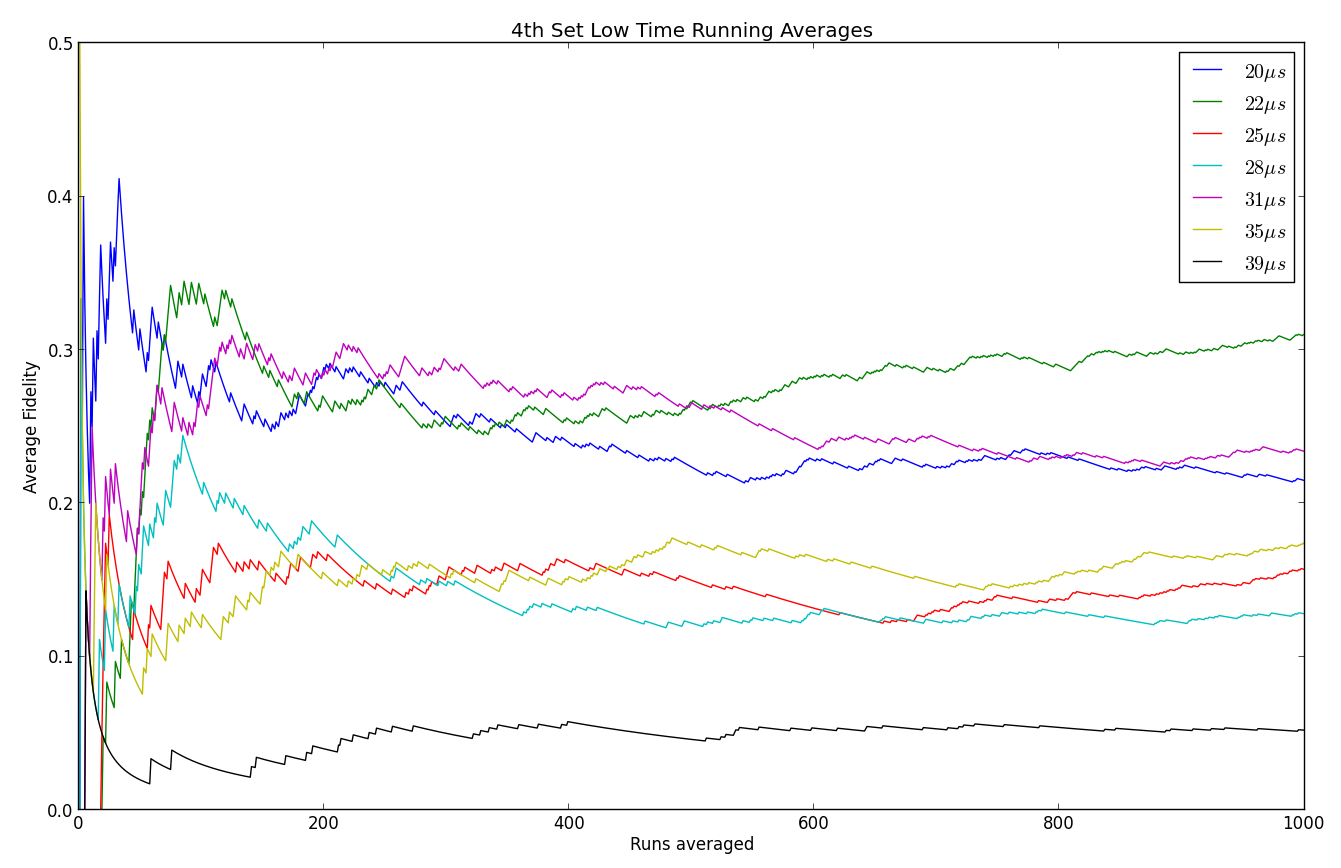
\includegraphics[bb= 0 0 1341 868]{img/4th_run_avg_low.png}
	}
	\caption[Running Fidelity Average]{Running average of the fidelity of the Hamiltonian ``6\_018'' for several short-time anneals, showing the change in fidelity with increasing read number.  The number of reads averaged over increases from zero to one thousand.  The rightmost edge of each data set shows the final fidelity estimate for that anneal time.  }
	\label{fig:running_avg}
\end{figure}
\section{Read noise}
First we examine the question of whether there is significant drift in the fidelity within a single run.  That is, does the probability of getting the ground state on any given read depend on the read number (the first read, second read etc.).  This question was examined on the Hamiltonian ``6\_018'' because the data collected on that particular Hamiltonian always consisted of at least 1000 reads per run.
Figure \ref{fig:running_avg} shows the running average of some short-time anneals from a single sweep of ``6\_018''.  If there is not significant read noise, we expect that the running average should flatten out and converge on the ``true'' fidelity after the appropriate number of reads.  For example, for a standard deviation $\sigma = \sqrt{np(1-p)}$ we expect that the running average should be within 5\% of the true fidelity after $\sim$ 200 reads.  Most of the anneal times appear to be reasonably flat past $\sim$ 500 reads, so the running averages appear to indicate to us that there isn't significant read noise (or at least, not nearly enough to be responsible for the short-time oscillations we saw in Chapter \ref{chap:prelim}).

The running average is a somewhat flawed quantity however, since it privileges earlier reads over later ones (since each read contributes like $1/N$ for $N$ reads already counted).  To remedy this we can also look at a rolling average of the fidelity as the reads come in.  Figure \ref{fig:rolling_avg} shows a rolling average of the fidelity for the same data as Figure \ref{fig:running_avg}.  Each point is the ground state fraction of the 100 reads around the labelled point; e.g. the value at point 500 is the number of ground states found from reads 450 to 550 over 100.  The rolling average has an advantage over the running average in that it does not prefer any part of the data set, but it can be harder to make out trends than in the running average.  It can be seen in the rolling average data that there does not appear to be a trend toward the fidelity being higher or lower in different segments of the run; e.g. the 22 $\mu$s run has highest fidelity in the nieghbourhood of read 600, while the 25 $\mu$s run has a minimum in the same location.

The combined results of the running and rolling averages would seem to indicate that intra-run errors, or errors occurring in the process of administering different reads, are not a significant contributor to the final observed fidelity for any given problem.

\begin{figure}
	\scalebox{0.35}{
		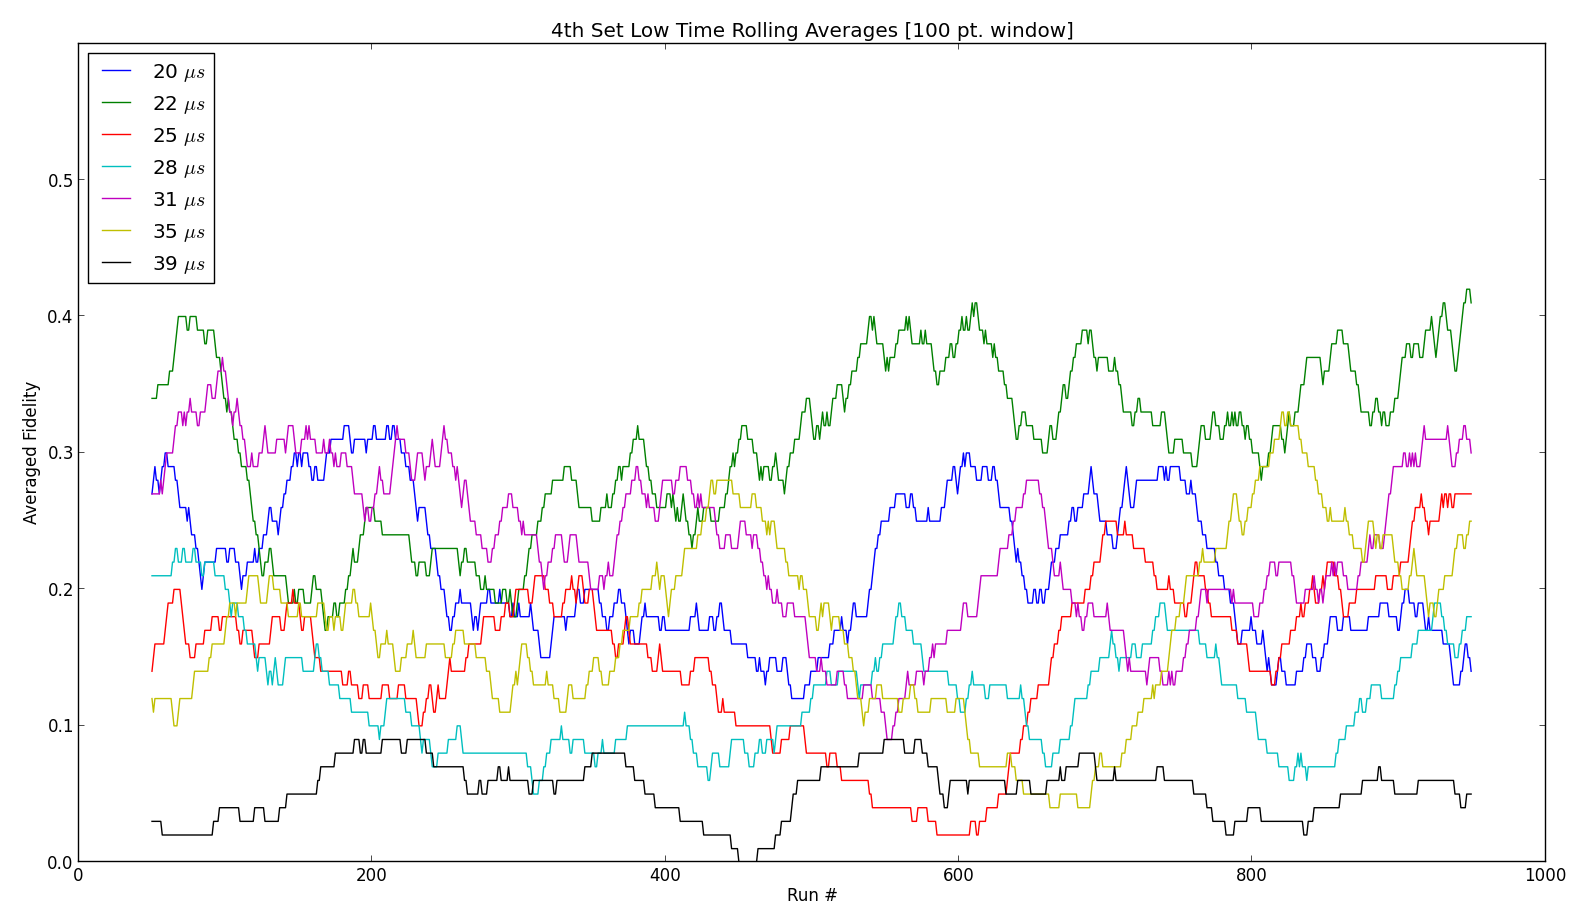
\includegraphics[bb=0 0 1582 917]{img/4th_run_roll_avg_low_100.png}
	}
	\caption[Rolling Fidelity Average]{Rolling average of the estimated fidelity for data collected from Hamiltonian ``6\_018'' at the seven shortest anneal times.  Each point is the average fidelity over a one hundred point window, e.g. the value at point 500 is the total number of times the ground state was measured between reads 450 and 550 divided by one hundred.}
	\label{fig:rolling_avg}
\end{figure}

\section{Short-Time Oscillations}
The Hamiltonian ``k44\_and'' was evaluated for times ranging from 20 $\mu$s to 20 ms, with 4 runs taken at each time point and 100 reads per run.  Figure \ref{fig:results_avg} shows these results.  Each run produced as estimated fidelity as in Chapter \ref{chap:prelim}, and the results shown here were synthesized by making a weighted average of each of the individual run's estimated fidelities.  The error bars shown here are the standard deviations of the means of the weighted averages, so small when the four runs produced nearly the same result and large when there was a large spread.  The short time oscillations are not entirely removed, although our estimates of the standard deviation matches up to the observed data much better; the trend of the data points falls almost entirely within the error bars.

\begin{figure}
	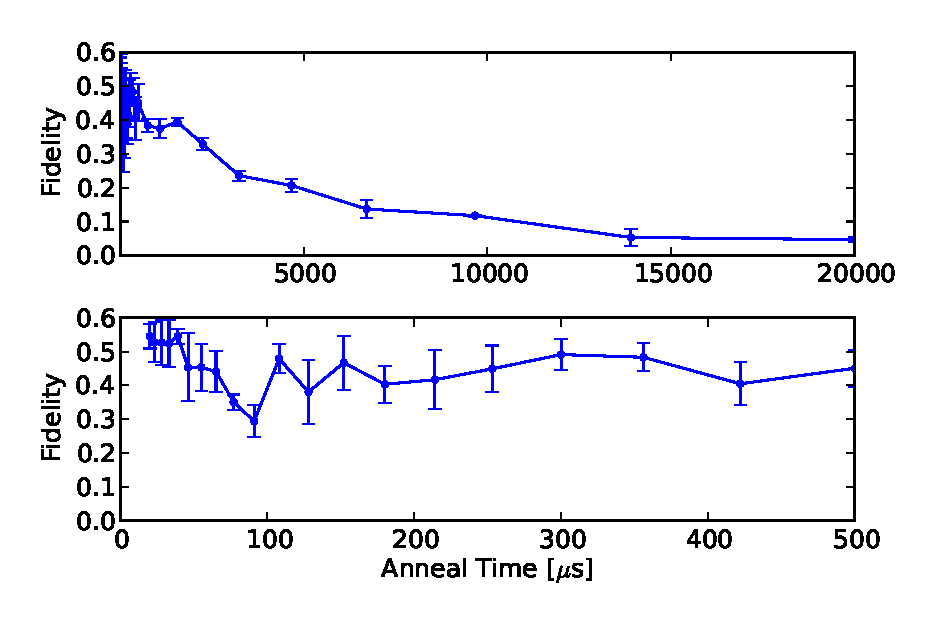
\includegraphics{img/final_single_k44.eps}
	\caption[Averaged Anneal Results]{Fidelity vs anneal time with each data point averaged over four different runs for the single qubyte ``k44\_and'' with a clone coupling value of -9.  Each run was used to estimate the fidelity independently as in Chapter \ref{chap:prelim}, with the final estimate the weighted average of each run.  The errorbars reflect the standard deviation of the distribution of estimates of the runs.}
	\label{fig:results_avg}
\end{figure}

\section{Clone coupling value}
\label{sec:coupling}

\begin{figure}
	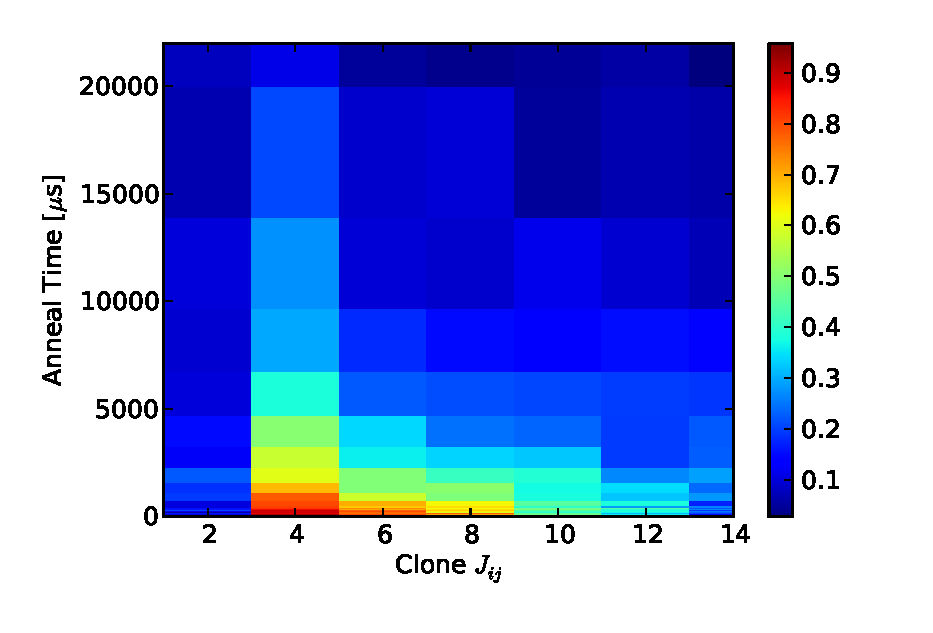
\includegraphics{img/n_8_t_v_c.eps}
	\caption[Variable Clone Coupling Fidelity]{Heat map of the fidelity as a function of anneal time and clone coupling value for the single qubyte ``k44\_and''.  The measured fidelity drops of rapidly with increasing clone coupling, but low clone coupling values do not preserve the ground state intact.  The sudden drop in fidelity at the smallest clone coupling value is caused by incorrect states with the same energy as the ground state.}
	\label{fig:clone_coupling}
\end{figure}

As discussed in Sections \ref{sec:embed_algo} and \ref{sec:resolution}, while for an ideal machine maximizing the clone coupling value would ensure that adding clones did not alter the ground states of our problem Hamiltonians, the \machine machine can only implement 15 different clone coupling values.  In addition, these values must be evenly spaced.  If we were to use a clone coupling value of $-14$ in a problem Hamiltonian which natively had coupling values of $-2,-1,1,2$, this would result in compressing each of the positive and negative couplings into one machine value.  The machine only implements couplings of the form 
\begin{equation}
	\pm\frac{x}{7}, 1 \le x \le 7
\end{equation}
so the above example would result in a physically implemented Hamiltonian of -1/7, -1/7, 1/7, $1/7$ in addition to the clone coupling of $-1$.  Most of the time this will result in a malformed Hamiltonian with incorrect ground states.

In addition to incorrect ground states, it is possible that the programming error in the machine is large enough to make the couplings $1/7$ and $2/7$ close enough to be likely to collide, whereas $1/7$ and $3/7$ could be far enough apart to be programmed correctly every time.  This could mean that even in scenarios where \machine has enough range to encode the problem Hamiltonian couplings correctly with a large clone coupling value we still don't want to do so.

This means that when selecting a clone coupling value we must balance these two competing factors, the desire to make the clone coupling as large as possible from a Hamiltonian correctness standpoint, and the desire to make it as small as possible from a machine resolution viewpoint.  The Hamiltonian correctness issue is correctness and knowable at the time the Hamiltonian is constructed; however in general to know whether a given clone coupling is large enough or not requires diagonalizing the Hamiltonian, and if this were possible then that would enable us to solve the initial computational problem directly.
The machine resolution problem is not necessarily the same from run to run; it could be that the compression of the problem Hamiltonian caused by the clone coupling value only makes it more likely for the machine to end up in an excited state.

\begin{figure}
	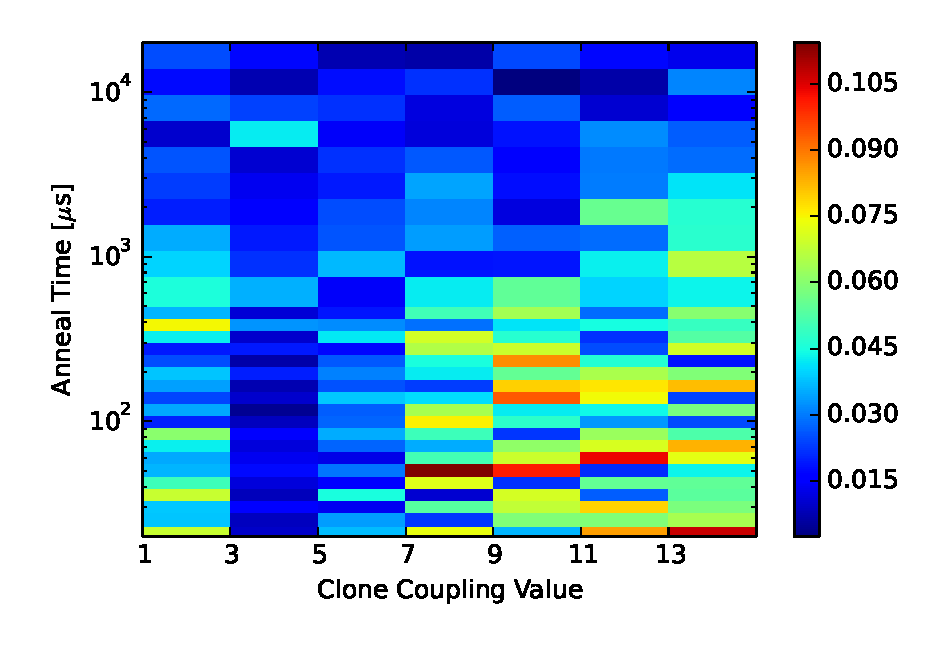
\includegraphics{img/t_c.eps}
	\caption[Fidelity Standard Deviation]{Heat map of the standard deviation of the estimated fidelity as a function of clone coupling value and annealing time for the single qubyte ``k44\_and''.  After $\sim$ 1000 $\mu$s the error drops down as we enter the long-time regime and the short-time oscillations die off.  The spread of the fidelity is also much lower for a clone coupling value of -3, which corresponds to the higher fidelities.}
	\label{fig:std_time}
\end{figure}

To empirically examine the impact of the value of the clone coupling, the ``k44\_and'' Hamiltonian was embedded multiple different times with a clone coupling value ranging from -1 to -14 (from the smallest coupling in the problem Hamiltonian to twice the native resolution of the machine).  Figure \ref{fig:clone_coupling} shows a heat map of the results of annealing these Hamiltonians from 20 $\mu$s to 20 ms.  Not only does fidelity increase as the clone coupling value is decreased, the short-time oscillations that we saw in Chapter \ref{chap:prelim} are removed.  This is shown very clearly in Figure \ref{fig:std_time}, which displays the standard deviation of the estimated fidelity as a function of anneal time and clone coupling value.

At longer anneal times the difference in fidelity is reduced, and the same long-time drop in fidelities that was observed in other Hamiltonians continues.  This means that the mechanism for the long-time fidelity drop is not strongly impacted by the clone coupling value.

The fidelity drops off strongly from its peak at a clone coupling value of -3.  Each of the higher clone coupling values corresponds to more and more compression of the computational couplings into fewer physical couplings.  This pattern does not continue to the -1 coupling, because that clone coupling value results in a malformed Hamiltonian where a domain wall forms in the ferromagnetic couplings, leading to what should be an excited state having the same energy as the ground state.  The ``k44\_and'' Hamiltonian's largest coupling value is $|3.0|$, which suggests that a clone coupling value of -3 performs well because it does not compress any couplings together.

\section{Size scaling}
The final property studied was the size scaling behaviour of ``k44\_and''.  This was done by translating the fields and couplings over to new qubytes.  The resulting Hamiltonian still only had one ground state, but was able to be scaled from 1 to 55 qubytes, a range of 8 to 440 spins.  Figure \ref{fig:time_spins} shows the fidelity plotted against anneal time and number of spins, for the clone coupling value which maximizes fidelity (-3).  The same plot for other clone couplings looks similar but with lower fidelity values across the board.  Larger Hamiltonians show similar behaviour to the original one qubyte ``k44\_and'', but fall off even faster with increased anneal time.

\begin{figure}
	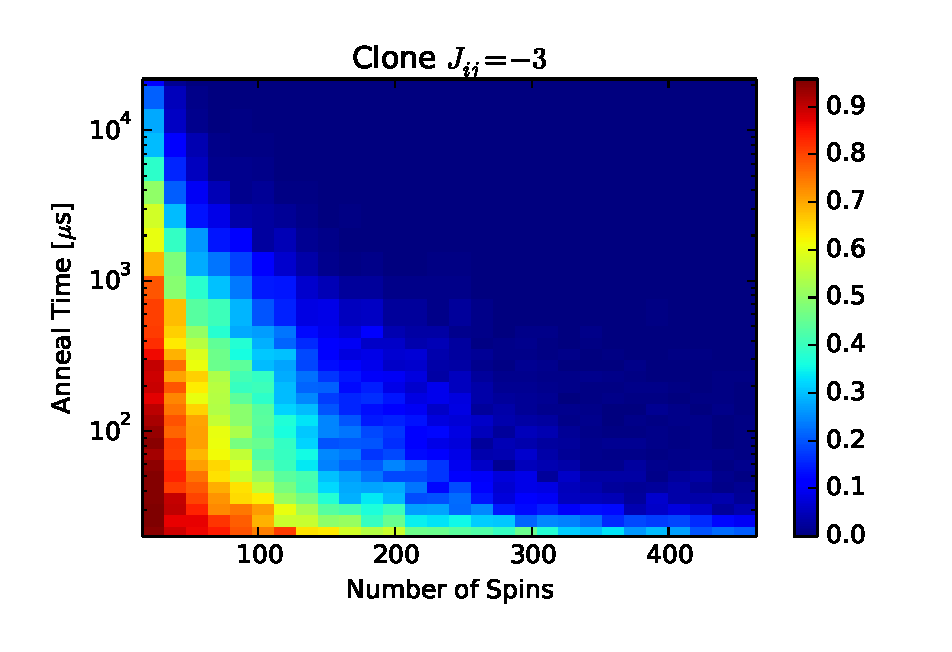
\includegraphics{img/pcolor_c_3.eps}
	\caption[Fidelity vs Time vs Number of Qubits]{Heat map of the estimated fidelity as a function of annealing time and number of spins in the Hamiltonian, with a clone coupling value of -3.}
	\label{fig:time_spins}
\end{figure}

\begin{figure}
	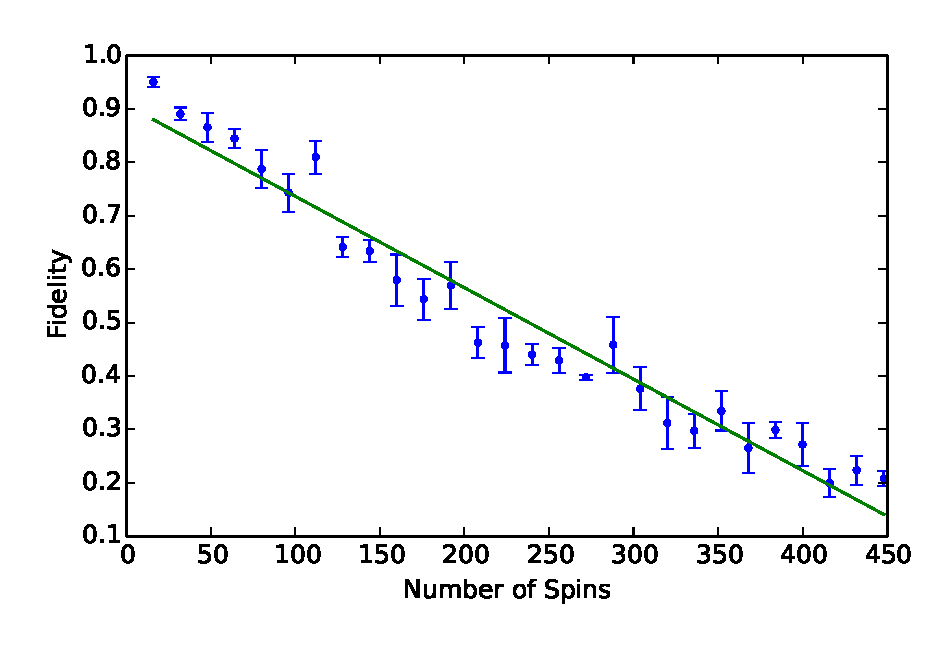
\includegraphics{img/trend.eps}
	\caption[Fidelity vs Number of Qubits]{Fidelity as a function of number of qubits for an anneal time of 20 $\mu$s and a clone coupling value of -3.  Green line shows line of best fit, with parameters: intercept of 0.91 and a slope of $-0.0017$.}
	\label{fig:trend}
\end{figure}

Figure \ref{fig:trend} shows the fidelity for annealing for 20 $\mu$s with a clone coupling value of -3 (that is, the values which maximize fidelity) as a function of number of spins.  The result is very close to a straight line; a linear regression is shown against the data.  This result would seem to indicate that for this problem, the \machine machine scales linearly.
